\documentclass[twoside]{article}
\usepackage{amsmath}
\usepackage{amsfonts}
\usepackage{graphicx}
\usepackage{color}

\setlength{\oddsidemargin}{0.25 in}
\setlength{\evensidemargin}{-0.25 in}
\setlength{\topmargin}{-0.6 in}
\setlength{\textwidth}{6.5 in}
\setlength{\textheight}{8.5 in}
\setlength{\headsep}{0.75 in}
\setlength{\parindent}{0 in}
\setlength{\parskip}{0.1 in}

\newcommand{\lecture}[3]{
   \pagestyle{myheadings}
   \thispagestyle{plain}
   \newpage
   \setcounter{page}{1}
   \noindent
   \begin{center}
   \framebox{
      \vbox{\vspace{2mm}
    \hbox to 6.28in {{\bf 10-708:~Probabilistic Graphical Models
10-708, Spring 2012 \hfill}}
       \vspace{6mm}
       \hbox to 6.28in {{\Large \hfill #1  \hfill}}
       \vspace{6mm}
       \hbox to 6.28in {{\it Lecturer: #2 \hfill Scribes: #3}}
      \vspace{2mm}}
   }
   \end{center}
   \markboth{#1}{#1}
   \vspace*{4mm}
}

\newcommand{\Dir}{\mathrm{Dir}}
\newcommand{\Gam}{\mathrm{Gamma}}
\newcommand{\Bet}{\mathrm{Beta}}
\newcommand{\DP}{\mathrm{DP}}
\newcommand\iid{\mathrel{\stackrel{\makebox[0pt]{\mbox{\normalfont\tiny iid}}}{\sim}}}
\newcommand{\todo}[1]{{\color{red} TODO: #1}}

\begin{document}

\lecture{Bayesian nonparametrics}{Sinead Williamson}{Victor Chahuneau, Rory Donovan, Abhimanu Kumar}

\section{Introduction}
Nonparametric models allow the number of parameters to grow with sample size.

\section{Nonparametric regression with Gaussian processes}
Usually, polynomial regression is used to model a set of points. Unfortunately, as the numbers of degree of freedom include, this produces overfitting.

\paragraph{The Gaussian distribution}
Two important properties: if $y=[y_1,y_2]$ is Gaussian, then:
\begin{itemize}
    \item the marginal $y_1$ is Gaussian
    \item the conditional $y_1 \mid y_2$ is Gaussian
\end{itemize}

\paragraph{The Gaussian process} A GP corresponds to a generalization of a $N$-variate Gaussian as $N \longrightarrow \infty$, such that the marginals are still normally distributed. It is thus a distribution over functions controlled by a covariance function.
Typically, an exponential kernel is used to define the covariance function.

\begin{figure}[htbp] %  figure placement: here, top, bottom, or page
   \centering
   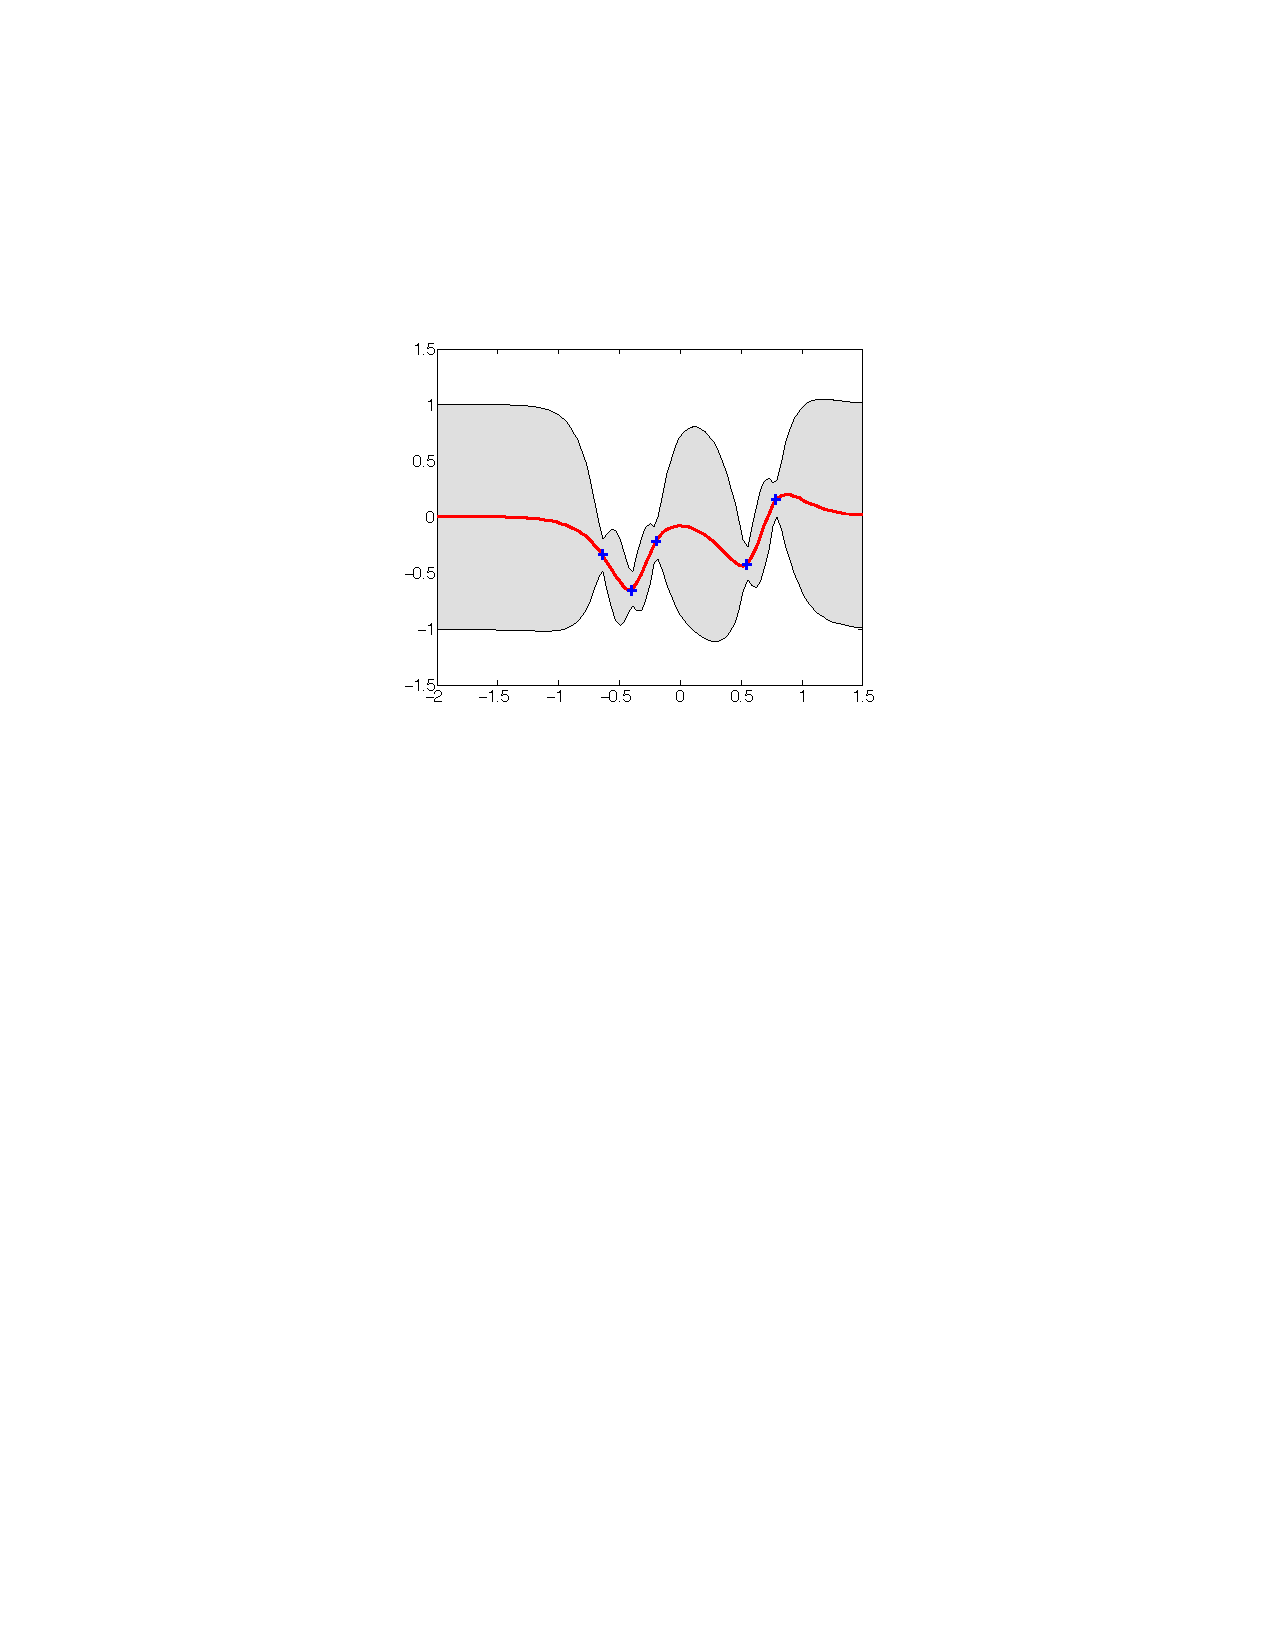
\includegraphics[width=0.5\textwidth]{gpinf.pdf} 
   \caption{Inference with the Gaussian process regression.  The predictions of the model are close to the existing data points and generic wherever data is absent.}
   \label{fig:gpinf}
\end{figure}

\section{Nonparametric mixture models}
\subsection{Finite mixture models}
Bayesian mixture models are obtained by putting a prior and integrating out.

\subsection{Properties of the Dirichlet distribution}
The $K$-dimensional Dirichlet distribution is given by
\[
\Dir(\alpha) = \frac{\prod_{k=1}^{K} \Gamma{(\alpha_k)}}{\Gamma{(\sum_{k=1}^{K} \alpha_k)}} \prod_{k=1}^{K} \pi_{k}^{\alpha_k - 1} \:,
\]

where $\alpha$ = $(\alpha_1, \dots, \alpha_K)$ is a vector of $K$ real numbers whose members must be non-negative, and the sum of which must be positive.  This vector controls where the probability mass is distributed over the $(K-1)$-dimensional unit simplex.  This can be seen by taking the excpectation of $\pi \sim \Dir(\alpha)$:
$$ \mathbb{E}(\pi_1 \dots \pi_K) = \frac{(\alpha_1 \dots \alpha_K)}{\sum_k \alpha_k} $$ 

An important property of the Dirichlet distribution is its conjugacy to the multinomial distribution. If $\theta \sim \Dir(\alpha_1,\ldots,\alpha_K)$ and $x_n \iid \theta$, then
\begin{align*}
  p(\pi \mid x_1, \dots, x_N)
  &\propto p(x_1, \dots, x_N \mid \pi) p(\pi) \\
  &= \left( \frac{\prod_{k=1}^{K} \Gamma{(\alpha_k)}}{\Gamma{(\sum_{k=1}^{K} \alpha_k)}} \prod_{k=1}^{K} \pi_{k}^{\alpha_k - 1} \right) \left( \frac{n!}{m_1! \ldots m_K!} \pi_1^{m_1} \ldots \pi_K^{m_K} \right) \\
  &\propto \frac{\prod_{k=1}^{K} \Gamma{(\alpha_k + m_k)}}{\Gamma{(\sum_{k=1}^{K} \alpha_k + m_k)}} \prod_{k=1}^{K} \pi_{k}^{\alpha_k + m_k - 1} \\
  &= \Dir(\pi \mid \alpha_1 + m_1, \dots, \alpha_K + m_K)
\end{align*}
 
In practice, this can be interpreted as smoothing the parameters.

The Dirichlet distribution is a distribution over distributions, defined by positive vectors which sum to one. A sample from a Dirichlet distribution $\pi \sim \Dir(\alpha)$ is itself a distribution over the parameter space (e.g. $\theta = (\mu, \Sigma) \in \mathbb{R}^n \times \mathbb{R}^{2n}$ for an $n$-variate Gaussian).

$$ p(x \mid \pi) = \sum_{k=1}^K \pi_k p(x \mid \theta_K) $$

\paragraph{Relation to the Gamma distribution}

\begin{itemize}
\item If $\eta_k \sim \Gam(\alpha_k, 1)$, then $\frac{(\eta_1,\ldots,\eta_K)}{\sum_k \eta_k} \sim \Dir(\alpha_1,\ldots,\alpha_K)$
\item If $\eta_1 \sim \Gam(\alpha_1, 1)$ and If $\eta_2 \sim \Gam(\alpha_2, 1)$, then
\[ \eta_1 +\eta_2 \sim \Gam(\alpha_1 + \alpha_2, 1) \]
\item Thus if $(\pi_1,\ldots,\pi_K) \sim \Dir(\alpha_1,\ldots,\alpha_K)$, then
\[ (\pi_1 + \pi_2,\ldots,\pi_K) \sim \Dir(\alpha_1 + \alpha_2, \alpha_3,\ldots,\alpha_K) \]
\end{itemize}

From the properties of the gamma distribution, we deduce that a $(K-1)$-dimensional Dirichlet distribution can be obtained from a $K$-dimensional Dirichlet distribution by summing the two first components.

\paragraph{Relation to the Beta distribution}
The Beta distribution is a Dirichlet distribution on the 1-simplex.
\begin{itemize}
\item If $(\pi_1,\ldots,\pi_K) \sim \Dir(\alpha_1,\ldots,\alpha_K)$ and $\theta \sim \Bet{(\alpha_1b,\alpha_1(1-b))}$, with $0 < b < 1$ then
\[ (\pi_1\theta,\pi_1(1-\theta),\pi_2,\ldots,\pi_K) \sim Dir{(\alpha_1 b,\alpha_1(1-b),\alpha_2,\ldots,\alpha_K)} \]
\item More generally, if $\theta \sim \Dir{(\alpha_1b_1,\ldots,\alpha_1b_N,\alpha_2,\ldots,\alpha_K)}$, then
\[ (\pi_1\theta_1,\ldots,\pi_1\theta_N,\pi_2,\ldots,\pi_k) \sim \Dir{(\alpha_1b_1,\ldots,\alpha_1b_N,\alpha_2,\ldots,\alpha_K)} \]
\end{itemize}


\paragraph{Renormalization Property}

If $(\pi_1,\ldots,\pi_K) \sim \Dir(\alpha_1,\ldots,\alpha_K)$, then
\[
\frac{(\pi_2,\ldots,\pi_K)}{\sum_{k=2}^K \pi_k} \sim \Dir(\alpha_2,\ldots,\alpha_K)
\]


\subsection{The Dirichlet process}
We can now generalize to an infinite number of parameters by splitting and renormalizing: $\pi \sim \Dir(\frac{\alpha}{K}), K \longrightarrow \infty$. This defines the Dirichlet process, which we write $G \sim \DP(\alpha, H)$, where $H$ is the base measure. Now the combination can be written:

$$ p(x \mid G) = \sum_{k=1}^K \pi_k p(x \mid \theta_K) $$

The concentration parameter $\alpha$ controls the sparsity of the distribution, and the base measure $H$ determines the locations of the atoms $\delta_{\theta_k}$.

More explicitly, 
\begin{itemize}
\item let $H$ be a distribution on some space $\Omega$, for example, a Gaussian distribution on over the reals.
\item let $\pi \sim \lim_{K \to \infty} \Dir{\left( \frac{\alpha_1}{K},\ldots,\frac{\alpha_K}{K} \right)}$
\item in the limit that $K \to \infty$, for $k = 1,\ldots,K$, let $\theta_k \sim H$
\item Then $G := \sum_{k=1}^{\infty}\pi_k \delta_{\theta_k}$ is an infinite distribution over H, and
\item we write $G \sim \DP{(\alpha,H)}$
\end{itemize}

\paragraph{Properties of the Dirichlet Process}
For any partition $A_1,...,A_K$ of $\Omega$, the total mass assigned to each partition is distributed according to $\Dir(\alpha H(A_1)),\ldots, \alpha H(A_K))$.

\todo{insert partition picture?}

\paragraph{Definition: finite marginals}
Another definition of the DP can be obtained by considering partitions of the probability space: A Dirichlet process is the unique distribution over probability distributions on some space $\Omega$, such that for any finite partition $A_1,...,A_K$ of $\Omega$
\[
\left( P(A_1),\ldots, P(A_K) \right) \sim \Dir{\left( \alpha H(A_1),\ldots, \alpha H(A_K) \right)}
\]

\paragraph{Conjugacy of the Dirichlet process}
The posterior over partitions given an observation $x$ is a finite dimensional Dirichlet :
$ G \mid x \sim \DP(\alpha+1, \frac{\alpha H + \delta_x}{\alpha + 1})$

\paragraph{The Dirichlet process as a predictive distribution}

The DP nonparametrically clusters observations: a new data point can either joint an existing cluster or a start a cluster of its own.  This data point trivially starts its own cluster, splitting the parameter space into the singleton (the $\theta_1$ cluster) and everything else.  Let $\pi_1$ be the atom at $\theta_1$.  Then the combined mass of all the other atoms is $1 - \pi_1$, and we have
\begin{itemize}
\item \emph{A priori} $(\pi_1,\pi_*) \sim \Dir(0,\alpha)$
\item \emph{A posteriori} $(\pi_1,\pi_*) \mid X_1 = \theta_1 \sim \Dir(1,\alpha)$
\end{itemize}

If we integrate out $\pi$, we get
\begin{align*}
   P(X_2 = \theta_k \mid X_1 = \theta_1)
&= \int P(X_2 = \theta_k \mid (\pi_1,\pi_*)) P(\pi_1,\pi_* \mid X_1=\theta_1) d\pi_1  \\
&= \int \Dir((\pi_1,1-\pi_1) \mid 1,\alpha) d\pi_1 \\
&= \mathbb{E}_{\Dir(1,\alpha)}[\pi_k] \\
&= \begin{cases}
    \frac{1}{1+\alpha} & \text{if } k=1,\\
    \frac{\alpha}{1+\alpha} & \text{for new } k.
\end{cases}
\end{align*}

In general, if $m_k$ is the number of memebers of cluster $k$, then if we have $K$ total clusters,
\begin{align*}
   P(X_{n+1} = \theta_k \mid X_1,\ldots,X_n)
&= \int P(X_{n+1} = \theta_k \mid \pi) P(\pi_1 \mid X_1,\ldots,X_n) d\pi  \\
&= \mathbb{E}_{\Dir(m_1,\ldots,m_K,\alpha)}[\pi_k] \\
&= \begin{cases}
    \frac{m_k}{1+\alpha} & \text{if } k<K,\\
    \frac{\alpha}{n+\alpha} & \text{for new } cluster.
\end{cases}
\end{align*}

With these probabilities for joining/starting a cluster, we tend to see a rich-get-richer effect, a hallmark of clustering schema and late-capitalism.

\todo{polya urn?}

\todo{chinese resaurant?}

\end{document}
